\documentclass[12pt,a4paper]{article}
\usepackage[utf8]{inputenc}
\usepackage[T1]{fontenc}
\usepackage{amsmath}
\usepackage{textcomp}

\usepackage{geometry}
\geometry{a4paper,left=25mm,right=25mm, top=2cm, bottom=2cm} 

\usepackage{graphicx} %fuer bilder

\usepackage{verbatim}




 \usepackage{mathptmx}
 \usepackage[scaled=.90]{helvet}
 \usepackage{courier}



\usepackage{listings}
\usepackage{color}
 
\definecolor{dkgreen}{rgb}{0,0.6,0}
\definecolor{gray}{rgb}{0.5,0.5,0.5}
\definecolor{mauve}{rgb}{0.58,0,0.82}

\pagestyle{empty}
\lstset{numbers=left, language=VHDL}
\lstset{showstringspaces=false,
basicstyle=\ttfamily\footnotesize,
breaklines=true,
tabsize=3,
commentstyle=\color{dkgreen},      % comment style
inputencoding={ansinew},
title=\lstname %zeigt titel der datei an
}

\usepackage{pdfpages} % fuer pdfs
\usepackage{hyperref} % fuer url


%keine einrückungen bei absatz
\parindent 0pt

\begin{document}
\title{Übung 01}
\author{Reinhard Penn, Bernhard Selymes}
\date{November 2015}

\normalsize

%Pfad zu c++ Dateien


%Beginn des Dokuments

\newcommand{\Uebung}{PROL16DE1}
\newcommand{\srcpath}{../../src}
\newcommand{\simpath}{../../sim}

%Angabe
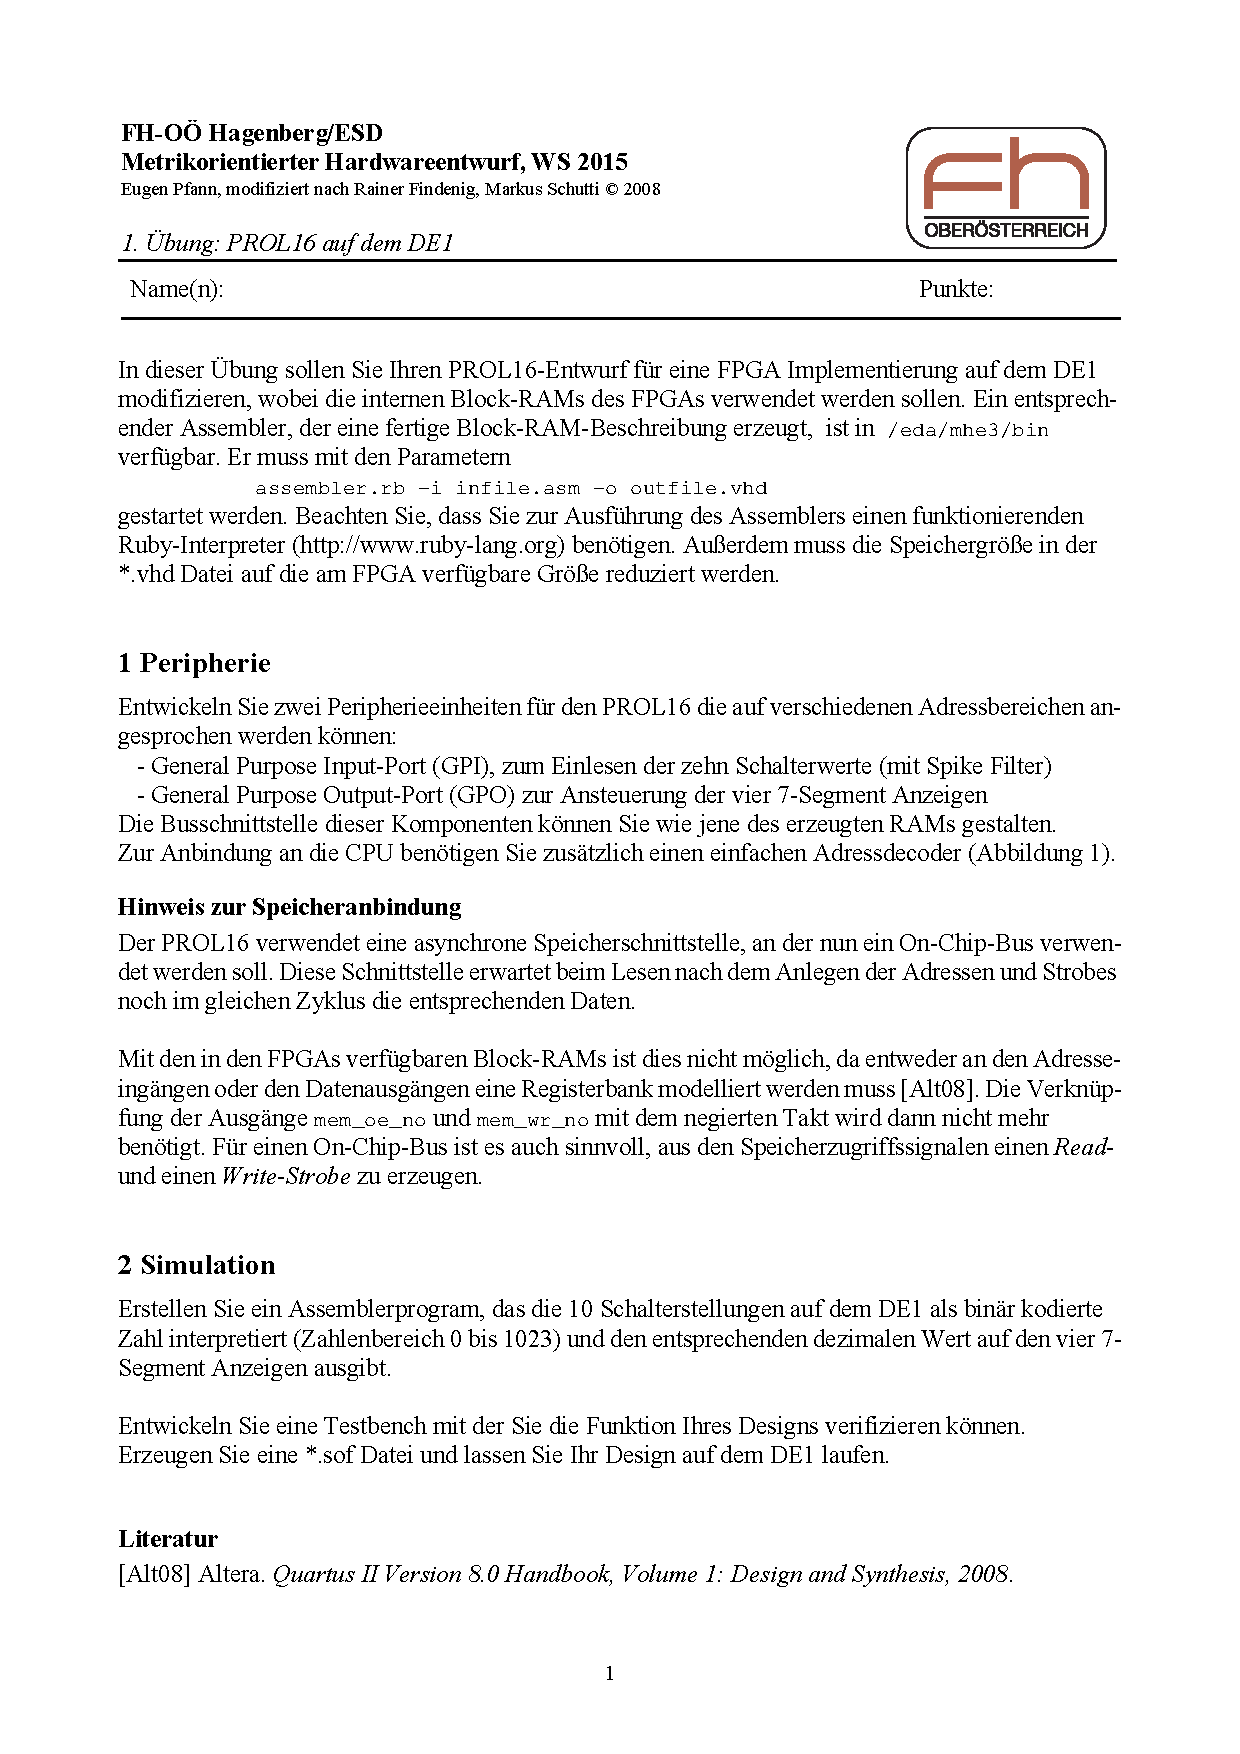
\includepdf[pages=-]{../Angabe.pdf}

\begin{center}
PROL16 auf dem DE1\\
Übungsprotokoll zur Übung 1\\
Metrikorientierter Hardwareentwurf\\
Bernhard Selymes, Reinhard Penn\\
11.11.2015
\end{center}


\section{Lösungsweg}
Das Assemblerprogramm wandelt die Binärwerte der Schalter in eine entsprechende BCD Darstellung um. Die Schalterwerte werden mithilfe von Load an der Adresse 3000 eingelesen, die BCD Werte für die Siebensegmentanzeige werden an die Adresse 3100 geschrieben.
Bei der Adresse 3000 leitet der Arbiter die Signale der Schalter als Daten an die CPU weiter. Bei der Adresse 3100 leitet der Arbiter die Daten der CPU an die Siebensegmentanzeige weiter.

\section{Source Code}
\subsection{Anpassung der Zuweisung der Memory Zugriffsignale in der CPU}
\lstinputlisting[linerange=108-110, firstnumber=108]{\srcpath/prol16/cpu.vhd}

\subsection{Auflösung der Adresssignale im Arbiter}
\lstinputlisting[linerange=25-35, firstnumber=25]{\srcpath/arbiter.vhd}

\subsection{Umwandlung binäre Codierung zu Siebensegment Anzeige}
\lstinputlisting[linerange=21-33, firstnumber=21]{\srcpath/bcd2sevsegment.vhd}

\subsection{Assemblerprogramm: Umwandlung von binär zu BCD}
\lstinputlisting[language=Ant]{\srcpath/convertToBCD.asm}

\section{Simulation}
Es wurde eine einfache Testbench gebaut in der im Stimuli Prozess verschiedene Schalterstellungen angelegt werden können. In der Waveform können dann die interessanten Signale überprüft werden.

\section{Synthese}
Es wurde ein einfaches Testbed angelegt, in dem die Polung der Siebensegementanzeige umgedreht wurde, da diese Ports low active sind.

\begin{figure}[ht]
\centering
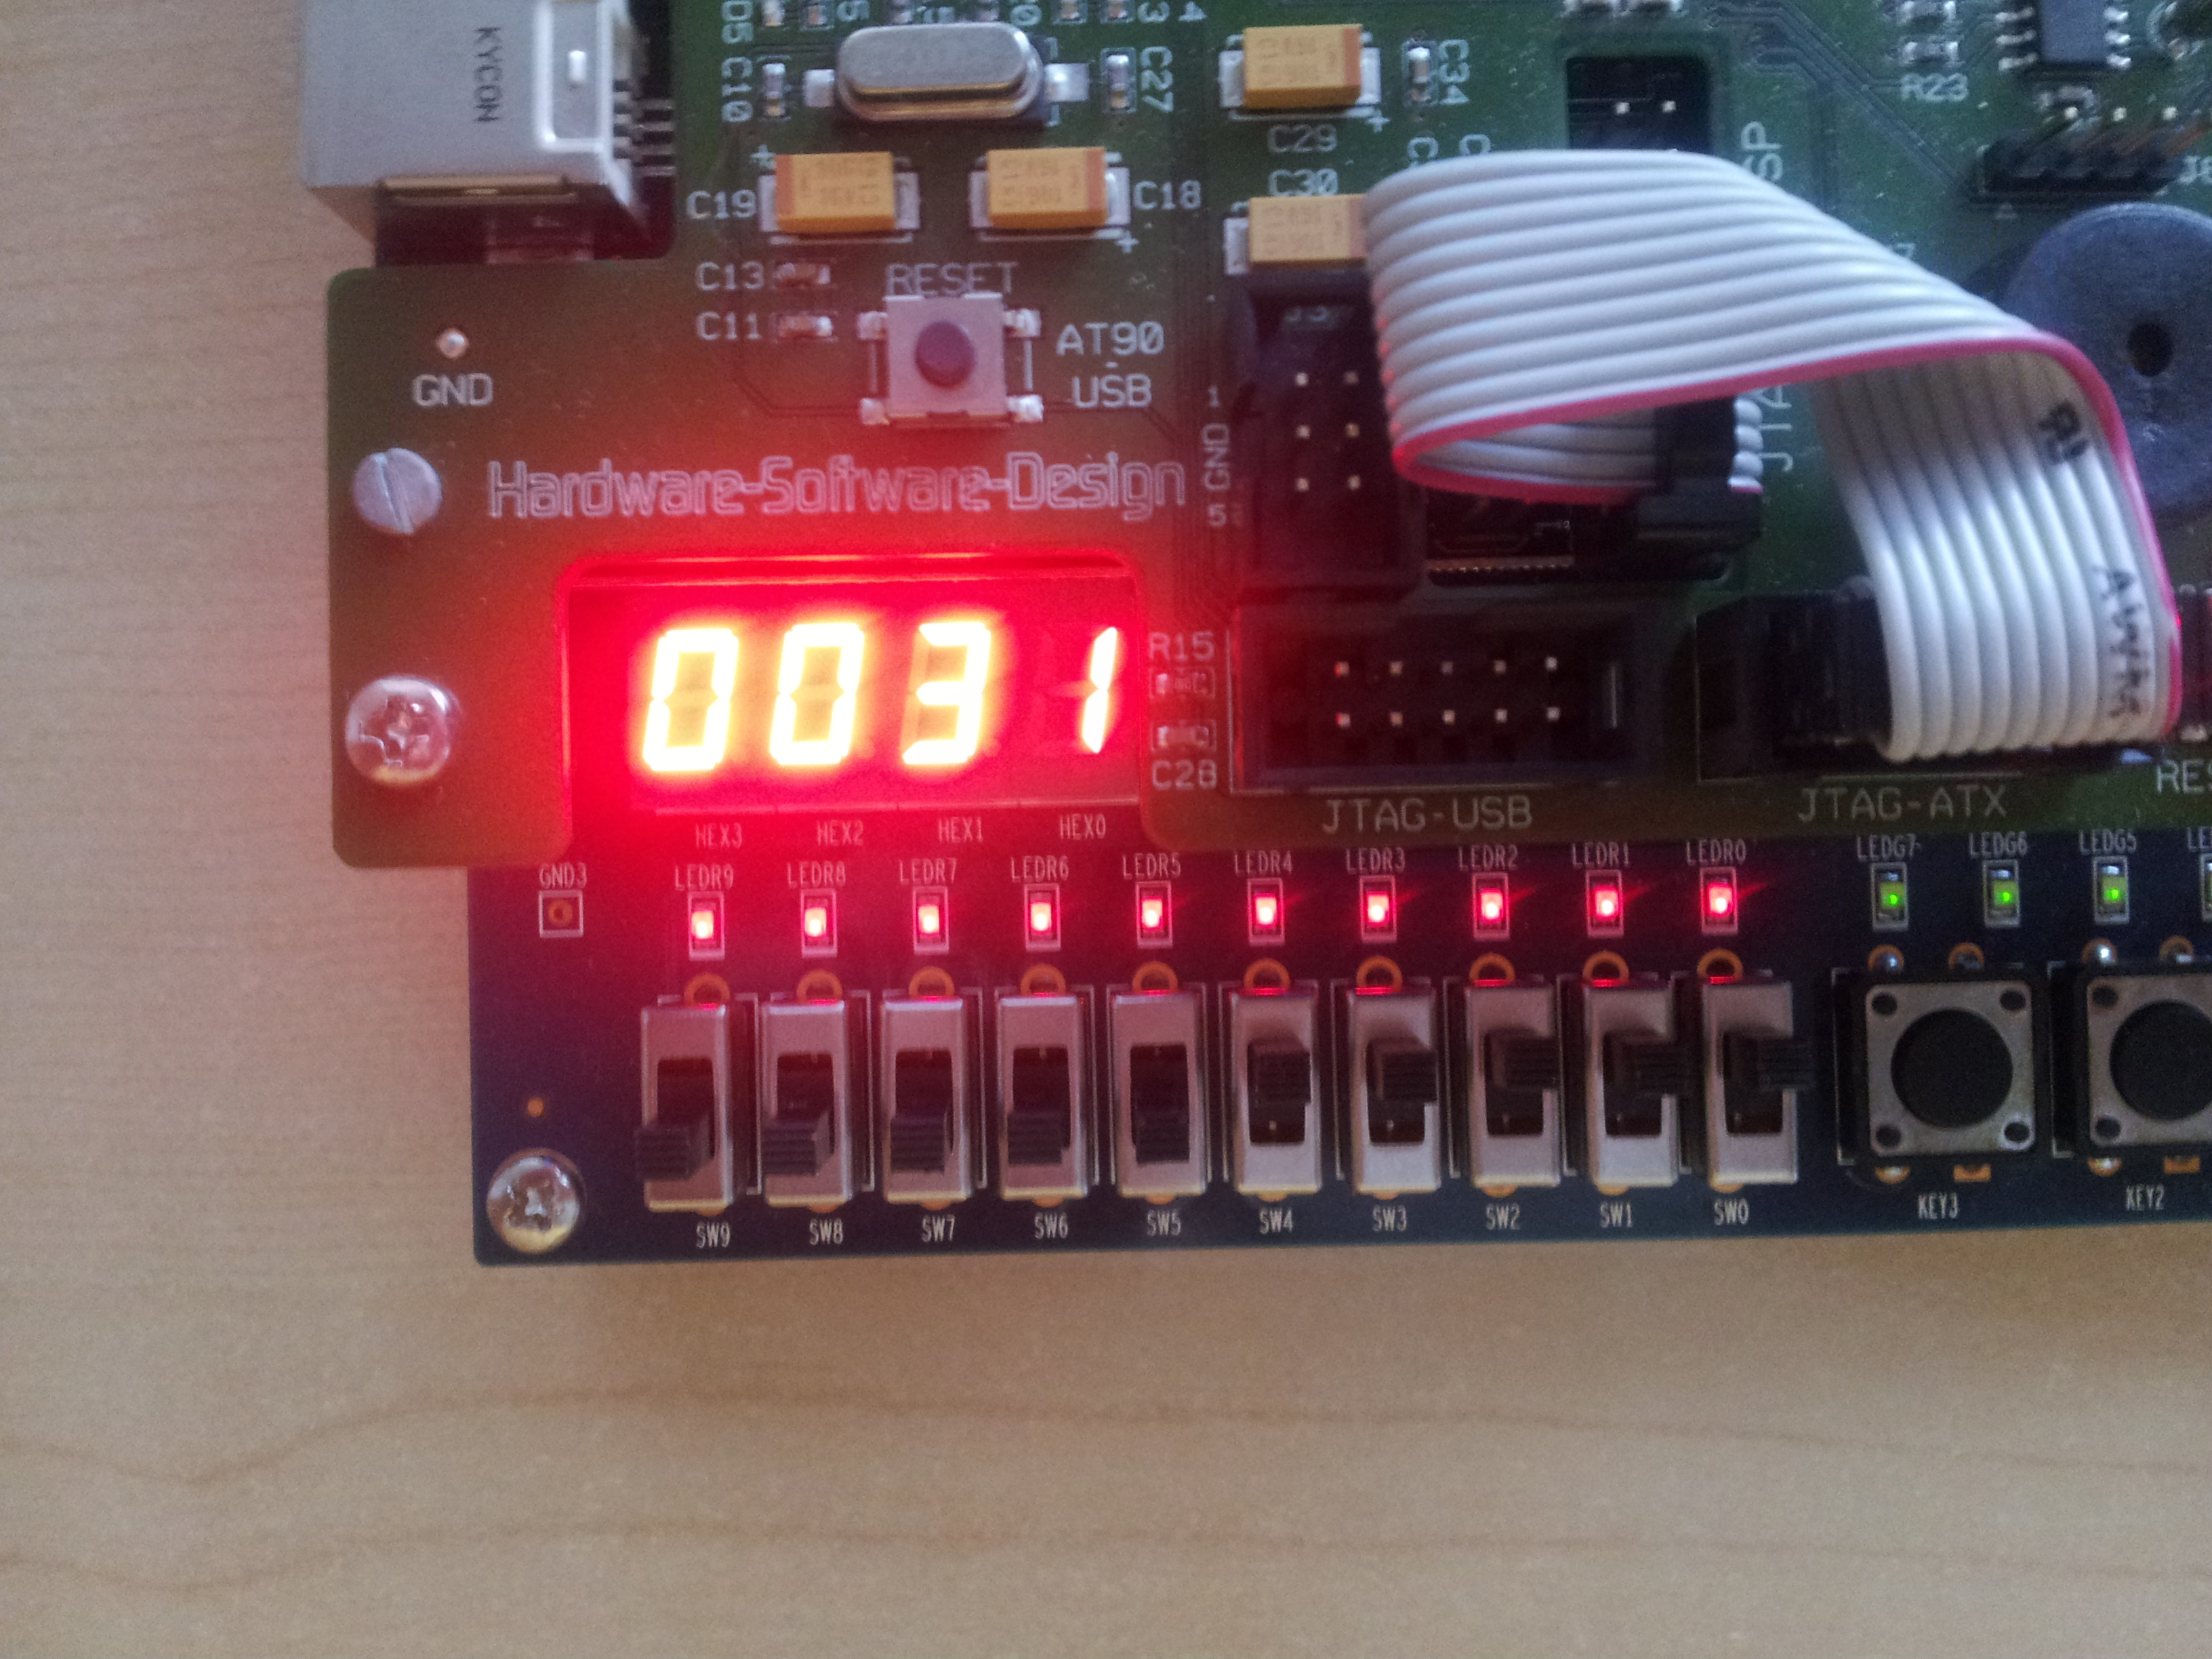
\includegraphics[width=\textwidth]{board}
\caption{Test auf dem Board.}
\end{figure}

\end{document}
